% Implementation sketch for the coauthor report, 2026-10-01; the supplement's copy
% (2026-10-07) drops the closing note, which its caption carries instead.
% Sources verified against:
%   benchmarks/17_use_case_acmg.sh: stage_derive, stage_convert, stage_link,
%       stage_govern, stage_query.
%   benchmarks/use_case/acmg/{use_case.json,generate.py,policy.ttl,carriers.rq}
%   benchmarks/use_case/acmg/{cohort/rare.rq,run_query.py}
%   vcf-rdfizer-wt-spdi (release/v3.3.0):
%       vcf_rdfizer_data/linkers/{spdi,ensembl-genes-grch38}/linker.ttl,
%       vcf_rdfizer_linking/runner.py, vcf_rdfizer_policies/engine.py.
% The linker consumes the same derived VCF as conversion, not conversion output.
% Only participant graphs/links enter policy evaluation; public annotations
% join the checked release at query time. Policies are not query rewriting.
% Build: pdflatex -interaction=nonstopmode -halt-on-error fig-linking-framework.tex
\documentclass[border=3pt]{standalone}
\usepackage[T1]{fontenc}
\usepackage{lmodern}
\usepackage{helvet}
\renewcommand{\familydefault}{\sfdefault}
\usepackage{tikz}
\usetikzlibrary{arrows.meta,calc,positioning}
\definecolor{teal}{HTML}{1F7F83}
\definecolor{tealbg}{HTML}{E8F3F2}
\definecolor{gold}{HTML}{A37B17}
\definecolor{goldbg}{HTML}{FBF2DB}
\definecolor{purple}{HTML}{5947A8}
\definecolor{purplebg}{HTML}{F0EDF9}
\definecolor{ink}{HTML}{26343D}
\definecolor{light}{HTML}{F3F5F6}
\newcommand{\codefont}[1]{{\ttfamily #1}}
\begin{document}
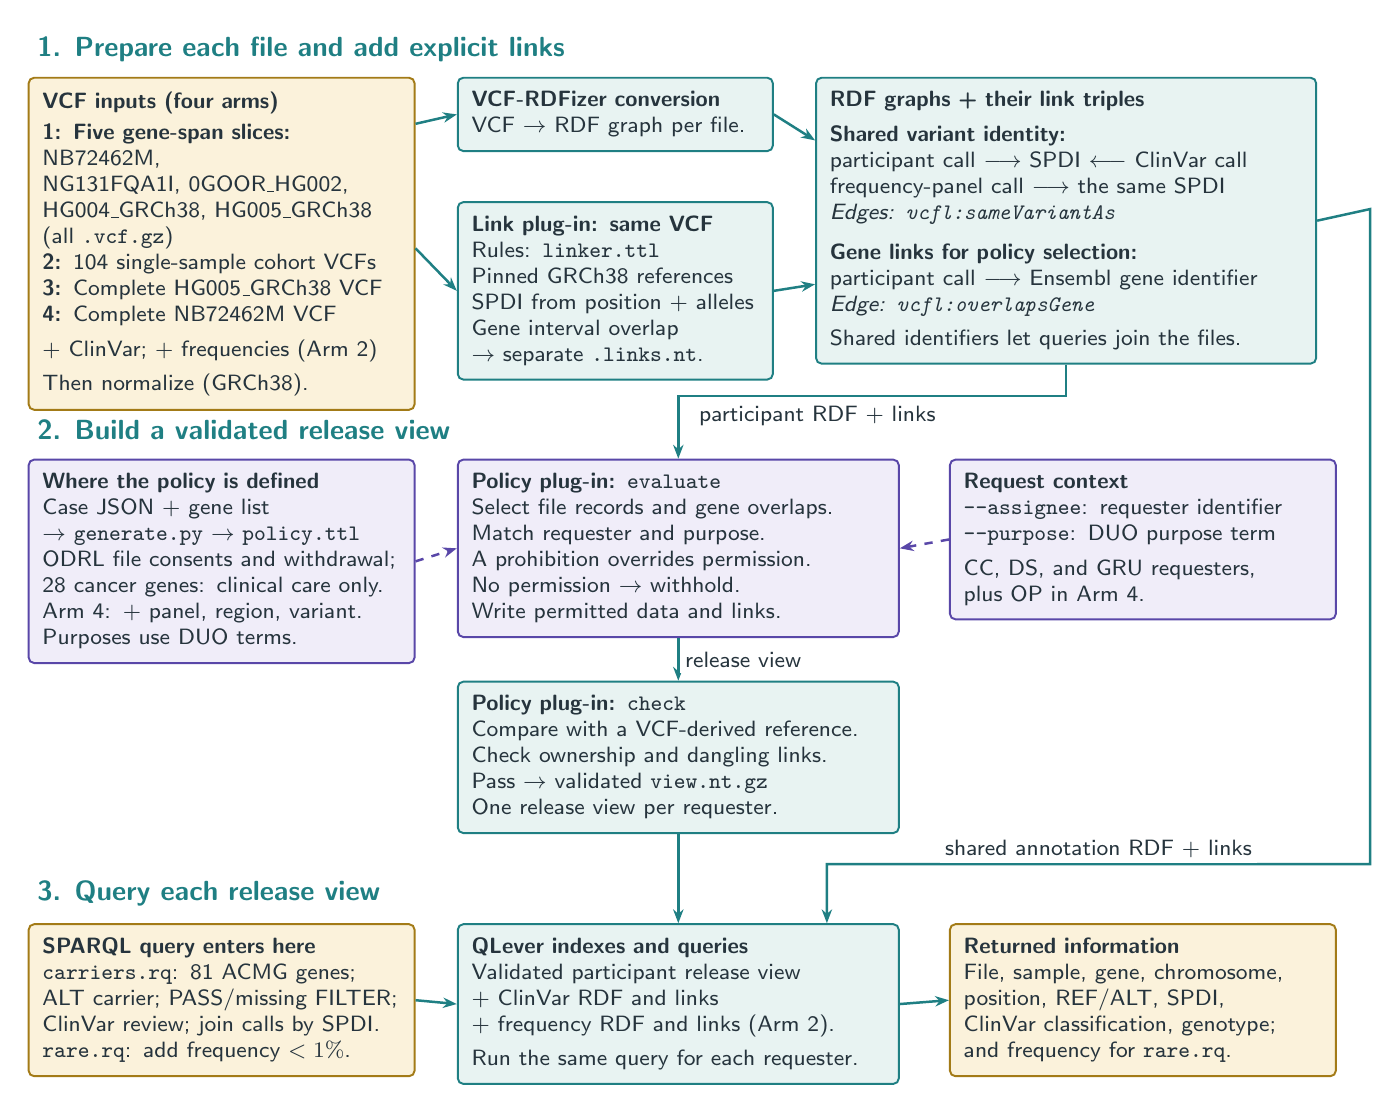
\begin{tikzpicture}[
  x=1cm,y=-1cm,
  font=\fontsize{8}{9.4}\selectfont, text=ink,
  box/.style={draw=teal,fill=tealbg,rounded corners=2pt,line width=.7pt,
    align=left,inner sep=5pt,anchor=north west,text width=#1},
  data/.style={draw=gold,fill=goldbg},
  policy/.style={draw=purple,fill=purplebg},
  flow/.style={-{Stealth[length=5pt]},draw=teal,line width=.9pt},
  control/.style={-{Stealth[length=5pt]},draw=purple,line width=.9pt,dashed},
  lab/.style={font=\fontsize{8}{9.5}\selectfont,fill=white,inner sep=2pt,align=center},
  stagehead/.style={font=\fontsize{10}{12}\selectfont\bfseries,text=teal,anchor=west}
]
\node[stagehead] at (0,0) {1. Prepare each file and add explicit links};

\node[box=4.55cm,data] (inputs) at (0,.35) {
  \textbf{VCF inputs (four arms)}\\[2pt]
  \textbf{1: Five gene-span slices:} NB72462M,\\
  NG131FQA1I, 0GOOR\_HG002,\\
  HG004\_GRCh38, HG005\_GRCh38\\
  (all \codefont{.vcf.gz})\\
  \textbf{2:} 104 single-sample cohort VCFs\\
  \textbf{3:} Complete HG005\_GRCh38 VCF\\
  \textbf{4:} Complete NB72462M VCF\\[3pt]
  + ClinVar; + frequencies (Arm 2)\\[3pt]
  Then normalize (GRCh38).
};
\node[box=3.65cm] (convert) at (5.45,.35) {
  \textbf{VCF-RDFizer conversion}\\
  VCF $\rightarrow$ RDF graph per file.
};
\node[box=3.65cm] (link) at (5.45,1.93) {
  \textbf{Link plug-in: same VCF}\\
  Rules: \codefont{linker.ttl}\\
  Pinned GRCh38 references\\
  SPDI from position + alleles\\
  Gene interval overlap\\
  $\rightarrow$ separate \codefont{.links.nt}.
};
\node[box=6.0cm] (graphs) at (10.0,.35) {
  \textbf{RDF graphs + their link triples}\\[3pt]
  \textbf{Shared variant identity:}\\
  participant call $\longrightarrow$ SPDI $\longleftarrow$ ClinVar call\\
  frequency-panel call $\longrightarrow$ the same SPDI\\
  \textit{Edges: \codefont{vcfl:sameVariantAs}}\\[5pt]
  \textbf{Gene links for policy selection:}\\
  participant call $\longrightarrow$ Ensembl gene identifier\\
  \textit{Edge: \codefont{vcfl:overlapsGene}}\\[3pt]
  Shared identifiers let queries join the files.
};

\draw[flow] ([yshift=-17pt]inputs.north east) -- (convert.west);
\draw[flow] ([yshift=-62pt]inputs.north east) -- (link.west);
\draw[flow] (convert.east) -- ([yshift=-23pt]graphs.north west);
\draw[flow] (link.east) -- ([yshift=-75pt]graphs.north west);

\node[stagehead] at (0,4.83) {2. Build a validated release view};
\node[box=4.55cm,policy] (policy) at (0,5.2) {
  \textbf{Where the policy is defined}\\
  Case JSON + gene list\\
  $\rightarrow$ \codefont{generate.py} $\rightarrow$ \codefont{policy.ttl}\\
  ODRL file consents and withdrawal;\\
  28 cancer genes: clinical care only.\\
  Arm 4: + panel, region, variant.\\
  Purposes use DUO terms.
};
\node[box=5.25cm,policy] (enforce) at (5.45,5.2) {
  \textbf{Policy plug-in: \codefont{evaluate}}\\
  Select file records and gene overlaps.\\
  Match requester and purpose.\\
  A prohibition overrides permission.\\
  No permission $\rightarrow$ withhold.\\
  Write permitted data and links.
};
\node[box=4.55cm,policy] (request) at (11.7,5.2) {
  \textbf{Request context}\\
  \codefont{-{}-assignee}: requester identifier\\
  \codefont{-{}-purpose}: DUO purpose term\\[3pt]
  CC, DS, and GRU requesters,\\
  plus OP in Arm 4.
};

\draw[flow] (graphs.south) -- ++(0,.4) -| (enforce.north);
\node[lab,anchor=west] at (8.45,4.66) {participant RDF + links};
\draw[control] (policy.east) -- (enforce.west);
\draw[control] (request.west) -- (enforce.east);

\node[box=5.25cm] (check) at (5.45,8.02) {
  \textbf{Policy plug-in: \codefont{check}}\\
  Compare with a VCF-derived reference.\\
  Check ownership and dangling links.\\
  Pass $\rightarrow$ validated \codefont{view.nt.gz}\\
  One release view per requester.
};
\draw[flow] (enforce.south) -- node[lab,right] {release view} (check.north);

\node[stagehead] at (0,10.72) {3. Query each release view};
\node[box=4.55cm,data] (query) at (0,11.1) {
  \textbf{SPARQL query enters here}\\
  \codefont{carriers.rq}: 81 ACMG genes;\\
  ALT carrier; PASS/missing FILTER;\\
  ClinVar review; join calls by SPDI.\\
  \codefont{rare.rq}: add frequency $<1\%$.
};
\node[box=5.25cm] (qlever) at (5.45,11.1) {
  \textbf{QLever indexes and queries}\\
  Validated participant release view\\
  + ClinVar RDF and links\\
  + frequency RDF and links (Arm 2).\\[3pt]
  Run the same query for each requester.
};
\node[box=4.55cm,data] (rows) at (11.7,11.1) {
  \textbf{Returned information}\\
  File, sample, gene, chromosome,\\
  position, REF/ALT, SPDI,\\
  ClinVar classification, genotype;\\
  and frequency for \codefont{rare.rq}.
};
\draw[flow] (check.south) -- (qlever.north);
\draw[flow] (query.east) -- (qlever.west);
\draw[flow] (qlever.east) -- (rows.west);

% Public annotations bypass participant policy filtering, then join at query time.
\draw[flow] (graphs.east) -- (17.05,2.03) -- (17.05,10.35)
  -- node[lab,above] {shared annotation RDF + links} (10.15,10.35)
  -- (10.15,11.1);

\end{tikzpicture}
\end{document}
